\documentclass{beamer}
\usepackage{stackengine}
\usepackage{mathtools}
\renewcommand\useanchorwidth{T}
\usepackage{xcolor}
\def\theyearwidth{1.5pt}
\def\mystrut{\rule{0ex}{.1ex}}
\def\myyrstrut{\rule[-1ex]{0ex}{2ex}}
\newlength\yrsfboxrule
\yrsfboxrule .4\fboxrule
\newcommand\yearwidth[1]{\def\theyearwidth{#1}\ignorespaces}
\newcommand\skipyears[2][black]{%
  \fboxrule\yrsfboxrule%
  \fboxsep=-\yrsfboxrule%
  \fcolorbox{#1}{#1}{\mystrut\hspace{#2}}%
  \ignorespaces%
}
\newcommand\showyear[2][black]{%
  \fboxsep=0pt%
  \stackunder[2pt]{%
    \colorbox{#1}{\myyrstrut\hspace{\theyearwidth}}%
  }{\tiny#2}%
  \ignorespaces%
}
\usetheme{Amsterdam}

\title{Approximation Algorithms for Stochastic Inventory Control Models}
\subtitle{A periodic-review stochastic inventory control problem}
\author[Hao Yuan, Feng Wei, Blake Miller]{Hao Yuan, Feng Wei, Blake Miller \\ {\ttfamily Github:\href{https://github.com/blakeapm/stochastic-inventory}{github.com/blakeapm/stochastic-inventory}}}
\date{\today}

\begin{document}
  \frame{\titlepage}
  \section{The Periodic-Review Stochastic Inventory Control Problem}
  \subsection{General Concepts}
  \begin{frame}
    \frametitle{The Periodic-Review Stochastic Inventory Control Problem}
    \begin{itemize}
      \item Computing a provably efficient inventory control policies is difficult because:
        \begin{itemize}
          \item demand per time-period is correlated
          \item demand is non-stationary (time-dependent, distribution changes with time)
          \item cost is hard to predict due to the nature of demand
        \end{itemize}
      \item Important for any company that seeks to minimize cost of holding excess inventory while minimizing backorder costs (unmet demand)
      \item Particularly important in industries where the demand environment is highly dynamic. (i.e. Apple's supply-chain for solid state drives, seasonal products such as rock salt)
      \item These environments experience high correlation between demands in different periods (difficult to compute optimal inventory policy).
    \end{itemize}
  \end{frame}
  \subsection{Minimizing Cost}
  \begin{frame}
    \frametitle{Minimizing Expected Cost}
    Our goal is to supply each unit of demand without ordering too early or too late. This is difficult because:
    \begin{itemize}
      \item Oftentimes demand and lead times (time between order and receipt of product) are unpredictable.
      \item Inaccuracies can be extremely costly, so it is important that approximations are provably accurate within a certain range of error
    \end{itemize}
    To illustrate the problem, a different, and simpler algorithm:
      \begin{center}
      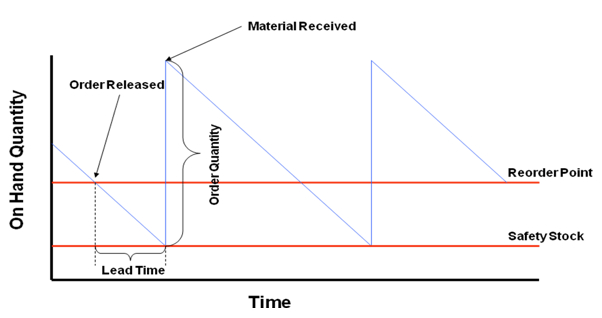
\includegraphics[height=1.5in]{purchasing.png}
      \end{center}
  \end{frame}

  \section{Expected Cost Function}
  \subsection{Minimizing Expected Cost}
  \begin{frame}
    \frametitle{Minimizing Expected Cost}
    \par
      {\centering\yearwidth{0.8pt}\tclap{\tiny t}\showyear{1}\skipyears[black]{.3in}\showyear{2}\skipyears[black]{.3in}\showyear{3}\skipyears[black]{.3in}\showyear{4}\skipyears[black]{.3in}\showyear{5}\skipyears[black]{.3in}\showyear{6}\skipyears[black]{.3in}$\text{  }\cdots\text{  }$\showyear{$T-1$}\skipyears[black]{.3in}\showyear{$T$}
    \par}
    \vspace{0.1in}
    At each time period in a a finite planning horizon of $T$ periods numbered $t=1,\cdots,T$, the following costs are incurred
    \begin{itemize}
      \item $c_t$: per-unit ordering cost at time $t$
      \item $h_t$: per-unit holding cost from $t$ to $t + 1$
      \item $p_t$: per-unit backlogging penalty at time $t$
      \item $NI_t$: net inventory at time $t$
    \end{itemize}
    The cost generated at time $t$ will be:
    \[C_t=c_tq_t+h_tNI_t^{+}+p_tNI_{t}^{-}\]
  \end{frame}
  \subsection{Parameters}
  \begin{frame}
    \frametitle{Expected Cost Function Parameters}
    To ensure the highest profit margin, we minimize the following function at each given time period:
    \begin{eqnarray*}
    V_{t}(x_{t},f_{t}) = \min_{x_{t}\leq y_{t}}\begin{cases}c_{t}(y_{t}-x_{t})+E[h_{t}(y_{t}-D_{t})^{+}+p_{t}(D_{t}-y_{t})^{-}|f_{t}]\end{cases}\\
    + E[V_{t+1}(y_{t}-D_{t},F_{t+1})|f_{t}]\}
    \end{eqnarray*}
    \begin{itemize}
      \item Cost periods $t,\cdots,T$
      \item $h_{t}\left(x_{t}+q_{t}-D_{t}\right)^{+} \text{is holding cost}$
      \item $p_{t}\left(x_{t}+q_{t}-D_{t}\right)^{-} \text{is backlogging cost}$
      \item $x_{t}$ is inventory position (how much inventory you have in stock and on order)
      \item $Q_{t}$ is the amount of product
      \item $D_{t}$ is the demand for the product (random)
      \item $c_{t}\left(q_{t}\right) \text{ is production cost}$
    \end{itemize}
  \end{frame}
  \subsection{Computational Challenges}
  \begin{frame}
  \frametitle{Computational Challenges}

  \end{frame}

  \section{The Algorithm and Computational Approaches}
    \subsection{Dynamic Programming}
    \begin{frame}
    \frametitle{Dynamic Programming}
      \begin{itemize}
        \item Let $V_{t}\left(x_{t}\right)$ be the optimal expected cost over over periods $t=t,\cdots,T.$
        \item Using dynamic programming, we can solve each $V_{t}$
        \item This approach would be accurate if it were feasible, but the term $E\left[V_{t+1}\left(x_{t}+q_{t}-D_{t}\right)\right]$ is very difficult to compute.
      \end{itemize}
    \end{frame}

    \subsection{Myopic (Na{\"i}ve) Approach}
    \begin{frame}
    \frametitle{Myopic (Na{\"i}ve) Approach}
      The myopic approach focuses only on minimizing the expected immediate cost that is going to be incurred in each period, while ignoring the cost over the rest of the horizon.
      \[c_{t}\left(q_{t}\right)+E\left[h_{t}\left(x_{t}+q_{t}-D_{t}\right)^{+}+p_{t}\left(x_{t}+q_{t}-D_{t}\right)^{-}\right]\]
    \end{frame}

    \subsection{Dual-Balancing Problem}
    \begin{frame}
    \frametitle{Dual-Balancing Problem}
      \[H_t^B(Q_t):=\sum\limits_{j=t+L}^T h_j(Q_t-(D_{[t,j]}-X_t)^+)^+\]
      \[\Pi_t^B:=p_t(D_{[t,t+L]}-(X_t^B+Q_t))^+=p_t(D_{[t,t+L]}-Y_t^B)^+\]
    \end{frame}

    \subsection{Why Dual-Balancing?}
    \begin{frame}
    \frametitle{Why Dual-Balancing?}

    \end{frame}
  \section{Coding and Implementation}
    \subsection{Coding and Implementation}
    \begin{frame}
    \frametitle{Coding and Implementation}

    \end{frame}
  \section{Results}
    \subsection{Time Complexity}
    \begin{frame}
    \frametitle{Time Complexity}
    Dual-balancing
    Myopic
    Dynamic Programming
    \end{frame}
    \subsection{Accuracy}
    \begin{frame}
    \frametitle{Accuracy}
    Dual-balancing vs. Myopic
    Dual-balancing vs. Dynamic Programming
    \end{frame}
  \section{Open Problems and Challenges in the Field of Stochastic Inventory Control}
    \subsection{Open Problems and Challenges in the Field of Stochastic Inventory Control}
    \begin{frame}
    \frametitle{Open Problems and Challenges in the Field of Stochastic Inventory Control}

    \end{frame}

\end{document}